\item Let $\mathbb{R}$ and $\mathbb{R}^3$ denote the set of real numbers and the three dimensional vector space over it, respectively. The value of $\alpha$ for which the set of vectors
\[
\{[2,-3,\alpha], \; [3,-1,3], \; [1,-5,7]\}
\]
does not form a basis of $\mathbb{R}^3$ is
 \hfill (EC 2024)
\item In the given circuit, the current $I_x$ (in mA) is
 \hfill (EC 2024)
\begin{figure}[H]\centering
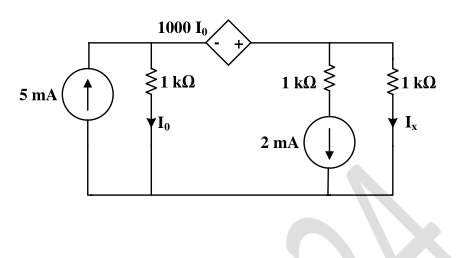
\includegraphics[width=0.65\columnwidth]{GATE/2024/EC/figs/q31.png}
\caption{}
\label{fig:q31}
\end{figure}
\item Consider the matrix
$
\begin{pmatrix}
1 & 2 \\
1 & k
\end{pmatrix},
$
where $k$ is a positive real number. Which of the following vectors is/are eigenvector(s) of this matrix?
 \hfill (EC 2024)
\begin{multicols}{4}
\begin{enumerate}
    \item $\myvec{1 \\ 2/k}$
    \item $\myvec{1 \\ 2/k}$
    \item $\myvec{2 \\ 1/k}$
    \item $\myvec{2 \\ -1/k}$
\end{enumerate}
\end{multicols}

